\documentclass[10pt,twocolumn,letterpaper]{article}

\usepackage{iccv}
\usepackage{times}
\usepackage{epsfig}
\usepackage{graphicx}
\usepackage{amsmath}
\usepackage{amssymb}

% Include other packages here, before hyperref.

% If you comment hyperref and then uncomment it, you should delete
% egpaper.aux before re-running latex.  (Or just hit 'q' on the first latex
% run, let it finish, and you should be clear).

\usepackage[pagebackref=true,breaklinks=true,letterpaper=true,colorlinks,bookmarks=false]{hyperref}

% \iccvfinalcopy % *** Uncomment this line for the final submission

\def\iccvPaperID{****} % *** Enter the ICCV Paper ID here
\def\httilde{\mbox{\tt\raisebox{-.5ex}{\symbol{126}}}}

% Pages are numbered in submission mode, and unnumbered in camera-ready
\ificcvfinal\pagestyle{empty}\fi

\begin{document}

  \title{Summary of Meshtalk WIP}

  \author{Jay\\
    CAU EAI Lab\\
    Lab address\\
    {https://yukinyaa.github.io}
  }
  \maketitle
  \thispagestyle{empty}

  \begin{abstract}
    The article summerises Meshtalk\cite{richard2021meshtalk}.
    The goal of this practice is to get familiar with \LaTeX{} and technical writing.
  \end{abstract}


  \section{Introuction to Meshtalk}
    Meshtalk is a generic method for generating full facial mesh animation from speech. It can generate 'lipsync' animation from a single frame of generic human facial mesh, and also can mix in emotional information from mesh animation.

    \subsection{Network Design}


      \begin{figure}[t]
        \begin{center}
        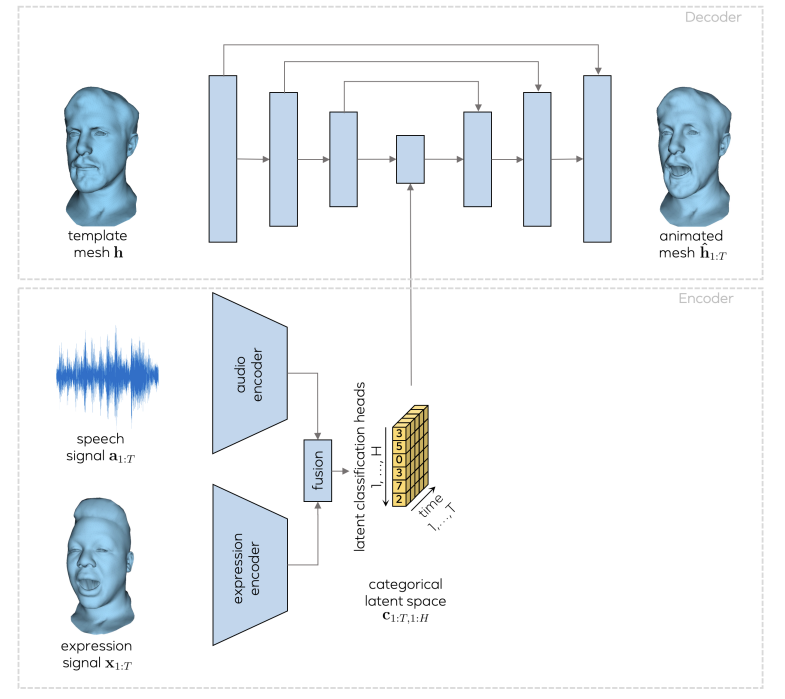
\includegraphics[width=0.8\linewidth]{meshtalk_overview.png}
        \end{center}
        \caption{The network diagram\cite{richard2021meshtalk}.}
        \label{fig:long}
        \label{fig:networkdiag}
      \end{figure}

      The network resembles Variational Autoencoder with multiple latent space as shown in Figure \ref{fig:networkdiag}.
      Target animation estimation \(\hat{h}\) is estimated from template mesh\(h\) by computing function \(\mathcal{D}\).
      \begin{equation}
        \hat{h}_{1:T} = \mathcal{D}(h, \mathsf{c}_{1:T, 1:H})
        \label{eq:1}
      \end{equation}
      \(c_{1:T}\) is a sequence of encoded latent space derived from audio sequence \(\mathsf{a}_{1:T}\) and expression signal mesh \(\mathsf{x}_{1:T}\)..
      \(c\) and \(a\) is first mapped to \(T*H*C\) dimentional latent space, then passed through Gumbel-softmax \cite{jang2017categorical} over every classification head.
      \begin{equation}
        \mathsf{c}_{1:T, 1:H} = [\mathsf{Gumbel}(\mathsf{enc}_{t,h,1:C})]_{1:T, 1:H}
      \end{equation}
      \begin{equation}
        \mathsf{enc}_{1:T,1:H,1:C} = \tilde{\xi}(x_{1:T}, a_{1:T}) 
      \end{equation}
      
    \subsection{Dataset}
      \begin{center}
        \begin{tabular}{c|c c}
          \hline
          Data Class | Resolution | Framerate
          \hline
          Face Mesh | 1,672 verticies | 30 FPS
          Audio | 16kHz | -
          Mel Spectogram | 80 Dimension | 10ms(100 Fps)
          \hline
      \end{center}
    \subsection{Training}
    The novel cross-modality loss is defined as
    \begin{equation}
      \begin{split}
        \mathcal{L}_{\mathsf{x}Mod} &= 
          \sum_{t=1}^{T}
          \sum_{v=1}^{V}
          \mathcal{M}_v^{\mathsf{(upper)}}
          (||\hat{h}_{t,v}^{\mathsf{(expr)}} - x_{t,v}||)\\
          &+
          \sum_{t=1}^{T}
          \sum_{v=1}^{V}
          \mathcal{M}_v^{\mathsf{(mouth)}}
          (||\hat{h}_{t,v}^{\mathsf{(audio)}} - x_{t,v}||)  
      \end{split}
    \end{equation}
    and loss for eye is defined as following.
    \begin{equation}
        \mathcal{L}_{\mathsf{eyelid}} = 
          \sum_{t=1}^{T}
          \sum_{v=1}^{V}
          \mathcal{M}_v^{\mathsf{(eyelid)}}
          (||\hat{h}_{t,v}^{\mathsf{(expr)}} - x_{t,v}||)
    \end{equation}
    \(\mathcal{M}^{(upper)}\) is a mask that assignes a higer weight to verticies around the mouth, and low weight to other.
    Correspondingly, \(\mathcal{M}^{(mouth)}\) is a mask that assignes a lower weright around the mouth, and vice versa.
    \(\mathcal{M}^{(eyelid)}\) is a specific eye loss, which was crucial.
    
    Final Loss term is defined as \(\mathcal{L} =\mathcal{L}_{\mathsf{x}Mod}+\mathcal{L}_{\mathsf{eyelid}} \), which gives both term equal weight.


%%%%%%%%%%%%%%%%%%%%%%% References %%%%%%%%%%%%%%%%%%%%%%%%%

{
  \small
  \bibliographystyle{ieee}
  \bibliography{ref}
}

\end{document}


